\documentclass[11pt,a4paper]{article}
\usepackage[a4paper,margin=2.5cm]{geometry}
\usepackage[utf8]{inputenc}
\usepackage[T1]{fontenc}
\usepackage[english]{babel}
\usepackage{microtype}
\usepackage{hyperref}
\usepackage{tikz}
\usetikzlibrary{arrows.meta,positioning,shapes.geometric}

\begin{document}

\noindent{\large\textbf{1.1.1 Conception Phase: Sentiment Analysis from News Articles}}\\[-1mm]
\noindent\textit{Alejandro Moral Aranda (ID: 92132071)}
\noindent\small\href{https://github.com/alejandromoralwork/sentiment-analysis}{GitHub: sentiment-analysis}
\vspace{2mm}

\textbf{Goal.}
The idea of the project is to check how a company is talked about in recent news. The app fetches articles by keyword, extracts the full text, cleans the text, runs sentiment analysis with three models, and stores the result so it can be viewed again later. The current version uses \href{https://fastapi.tiangolo.com/}{FastAPI} for the backend, \href{https://newsapi.org/}{NewsAPI} for the news source, and \href{https://www.crummy.com/software/BeautifulSoup/bs4/doc/}{BeautifulSoup} for text cleanup. The frontend is a small HTML and JavaScript dashboard that shows the live result.

\textbf{Main idea of the system.}
\begin{center}
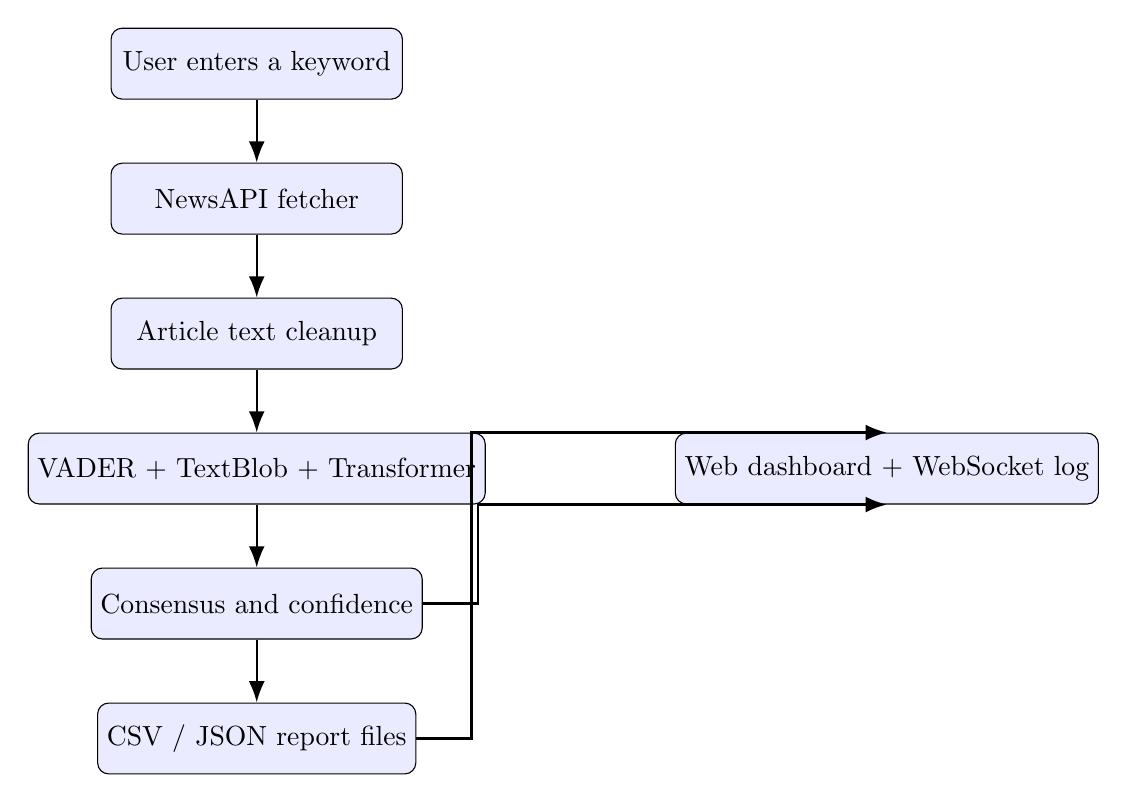
\begin{tikzpicture}[
    node distance=0.8cm,
    block/.style={rectangle, rounded corners, draw=black, fill=blue!8, minimum width=3.7cm, minimum height=0.9cm, align=center},
    arrow/.style={-{Latex[length=2.7mm]}, thick}
]
\node[block] (start) {User enters a keyword};
\node[block, below=of start] (fetch) {NewsAPI fetcher};
\node[block, below=of fetch] (clean) {Article text cleanup};
\node[block, below=of clean] (models) {VADER + TextBlob + Transformer};
\node[block, below=of models] (vote) {Consensus and confidence};
\node[block, below=of vote] (save) {CSV / JSON report files};
\node[block, right=2.4cm of models] (ui) {Web dashboard + WebSocket log};

\draw[arrow] (start) -- (fetch);
\draw[arrow] (fetch) -- (clean);
\draw[arrow] (clean) -- (models);
\draw[arrow] (models) -- (vote);
\draw[arrow] (vote) -- (save);
\draw[arrow] (vote.east) -- ++(0.7,0) |- (ui.south);
\draw[arrow] (save.east) -- ++(0.7,0) |- (ui.north);
\end{tikzpicture}
\end{center}

\textbf{Component overview.}
\begin{itemize}
    \item The frontend is a small dashboard in HTML and JavaScript with live WebSocket updates.
    \item The backend is a FastAPI app with a WebSocket channel for live progress messages.
    \item News articles are fetched from NewsAPI and then parsed with BeautifulSoup.
    \item Sentiment is checked with VADER, TextBlob, and a RoBERTa transformer model.
    \item The text is cleaned before analysis so URLs, emails, and extra noise do not affect the result too much.
    \item Reports are saved in \texttt{data/reports/} as JSON and CSV files.
\end{itemize}

\textbf{Why this structure.}
News articles are long and sometimes messy, so the system needs a few steps before classification. First the article is fetched, then the HTML is cleaned, and after that the sentiment models run on the text. This is better than only checking the headline, because headlines often miss the real meaning. Using a cleaned article body plus the headline gives the models more useful context.

\textbf{Validation idea.}
The project is not treated like a black box. The output from VADER, TextBlob, and the RoBERTa model is compared with each other, and the final report shows where the models agree or disagree. That way it is easier to see when the result is stable and when it is not. The report also includes a simple confidence value based on how many models agree.

\textbf{Planned implementation choice.}
The project is built in Python because the needed libraries are easy to use together. The backend keeps the logic in small modules: article fetching, text cleaning, sentiment analysis, and report saving. This makes the code easier to read and also easier to change later if a better model or source is needed.

\textbf{Short conclusion.}
The conception phase ended with a simple but working plan: fetch news, clean the text, run three sentiment models, compare the result, and save everything in a report that can be loaded again in the browser.

\vspace{2mm}
\textbf{Project updates (implementation notes).}
During implementation the project was extended to include a command-line runner and packaging notes so the tool can be delivered as a standalone executable for non-technical users (marketing). The codebase now uses structured logging, a pinned example requirements file for reproducible installs, and separate developer and user guides located in the `docs/` folder. A small build script (`build_exe.bat`) and `cli.py` were added to simplify creating a Windows EXE for distribution.

\end{document}
